\documentclass[12pt]{article}
\usepackage[utf8]{inputenc}

% Importing settings from setup.sty
\usepackage{setup}
\usepackage{booktabs}
\usepackage{multicol}
\usepackage{multirow}
\usepackage{glossaries}
% \makenoidxglossaries
% \newcommand{\prox}{\operatorname{prox}}


% \pagenumbering{roman}
\begin{document}

% Inserting title page
\import{./}{title}

\pagenumbering{gobble}
\tableofcontents
% \listoffigures
% \listoftables



\newgeometry{
  left=25mm,
  right=25mm,
  top=25mm,
  bottom=25mm}
\pagenumbering{arabic}

\section{Introduction}
``Learning without data collection'' is a provocative way to describe the process of learning from a single, or very few example. Humans however, are able to learn in such a way. Algorithms on the other hand, especially deep learning ones, are very data-hungry even for simple tasks such as recognising a cat from a dog. \\
In this paper, we will discuss several high-level, almost philosophical, directions that may not be used to their full potential. We will use an approach that relies on biomimicry. Biomimicry is the practice of studying nature's systems, processes, and designs to inspire and inform the development of human-made technologies, products, and innovations. It involves observing and learning from nature's strategies for problem-solving, adaptation, and sustainability and then applying these insights to create more efficient and effective solutions to human challenges. \\
We will first introduce the concept of Motion Invariance, as well as a short motivation for its use.

\section{Motion Invariance}
\label{sec: motion invariance}
In this section, we will give some context to the notion of learning without data collection and we will introduce the notion of motion invariance. We will see that motion invariance turns out to be quite useful in terms of efficiency, especially when Human performance is compared to deep learning algorithms.

\subsection{A bit of context}
Learning without data collection can be applied to many fields within machine learning. One notable example is the field of computer vision. When humans see a object moving, they are almost imidiately able to recognise it. We do not require hundreds of thousands of examples in order to identify it. One iteresting thing however is that, when we see a paused video, on a phone or a computer screen for instance, we are sometimes incapable of recognising objects. Think of a paused video about a jaguar in the jungle. The jaguar may be partially, or almost completely hidden. In this case, it may be difficult to identify it. When we turn the video on, it may still be challenging to see the jaguar if he is immobile. However, as soon as the jaguar starts moving, we are able to identify it. This is because of motion invariance \cite{gori2022}, which informs us of the consistency of an object (the jaguar in this case) through time.

\subsection{The concept of Motion Invariance}
Indeed, we know that the paws, the ears, the tail and all other body parts of the jaguar will not start splitting up or drastically changing shape as time goes. By the principles of motion invariance, nature somehow gives us a huge amount of information at one, for free. This hints that the current state of the art in computer vision is far from the best we can achieve, as it is already far from human level with respect to data efficiency. We can note that on the one hand, deep learning already beats the best medical doctors when it comes to detecting some types of cancer \cite{shen2019}. On the other hand however, as deep learning requires large quantities of data, humans are more efficient in this regard. As such, we arrive to the somewhat contradictory conclusion that \textit{deep learning is both better-performing (in terms of accuracy) and worse-performing (in terms of data efficiency) than humans}.

\section{Focus of attention: Motion Invariance is not all you need}
We saw in section \ref{sec: motion invariance} that motion invariance is a gift of nature that Humans are able to use to achieve better efficiency than deep learning algorithms, although with large quantities of data such algorithms are sometimes able to outperform humans. In this section, we will see that motion invariance also has its flaws: although it may be necessary, it is not sufficient for perfect recognition in all cases.

\subsection{Motion invariance is not sufficient}
In the example of the jaguar considered previously, we see that motion invariance is not sufficient. Indeed, it requires that the object is moving. If the object is not moving, motion invariance will not be able to help us. This is because motion invariance is a property of the object as it goes through time. Let us consider a famous pathological example of the flaws of motion invariance \cite{gori2022}. Due to the biological properties of its vision, a frog is not able to see what does not move. As a result, a frog could be surrounded by food and still starve to death if the food is immobile. This example illustrates the fact that there has to be more than just motion invariance to achieve perfect recognition. One other important element is the notion of attention, in the sense that we need to focus on the right part of the image in order to recognise the object. 

\subsection{The concept of Focus of Attention}
\subsubsection{Introduction to the focus of attention}
The concept of attention is illustrated by the natural phenomenon of the focus of attention. The concept of \textbf{focus of attention} refers to the ability to selectively concentrate on specific aspects of the visual scene. This is to some extent what Convolutional Neural Networks \cite{lecun1995} and transformers \cite{vaswani2017} intend to do, but the amount of data needed for these networks to perform well demonstrates that we are still very far from the Holy Grail of (at least) human-level efficiency. \\
The human capability to use the focus of attention is allowed by the cones in our eyes. These cones are responsible for the color vision. They are able to detect the presence of a specific color in a given area of the visual field (somehow like channels in a Convolutional Neural Network).

\subsubsection{The duck-rabbit illusion}
The duck-rabbit illusion is a famous ambiguous image in which both a duck and a rabbit can be seen, depending on one's point of view. An illustration of the duck-rabbit illusion is provided in figure \ref{fig: duck-rabbit}.
\begin{figure}[ht]
  \centering
  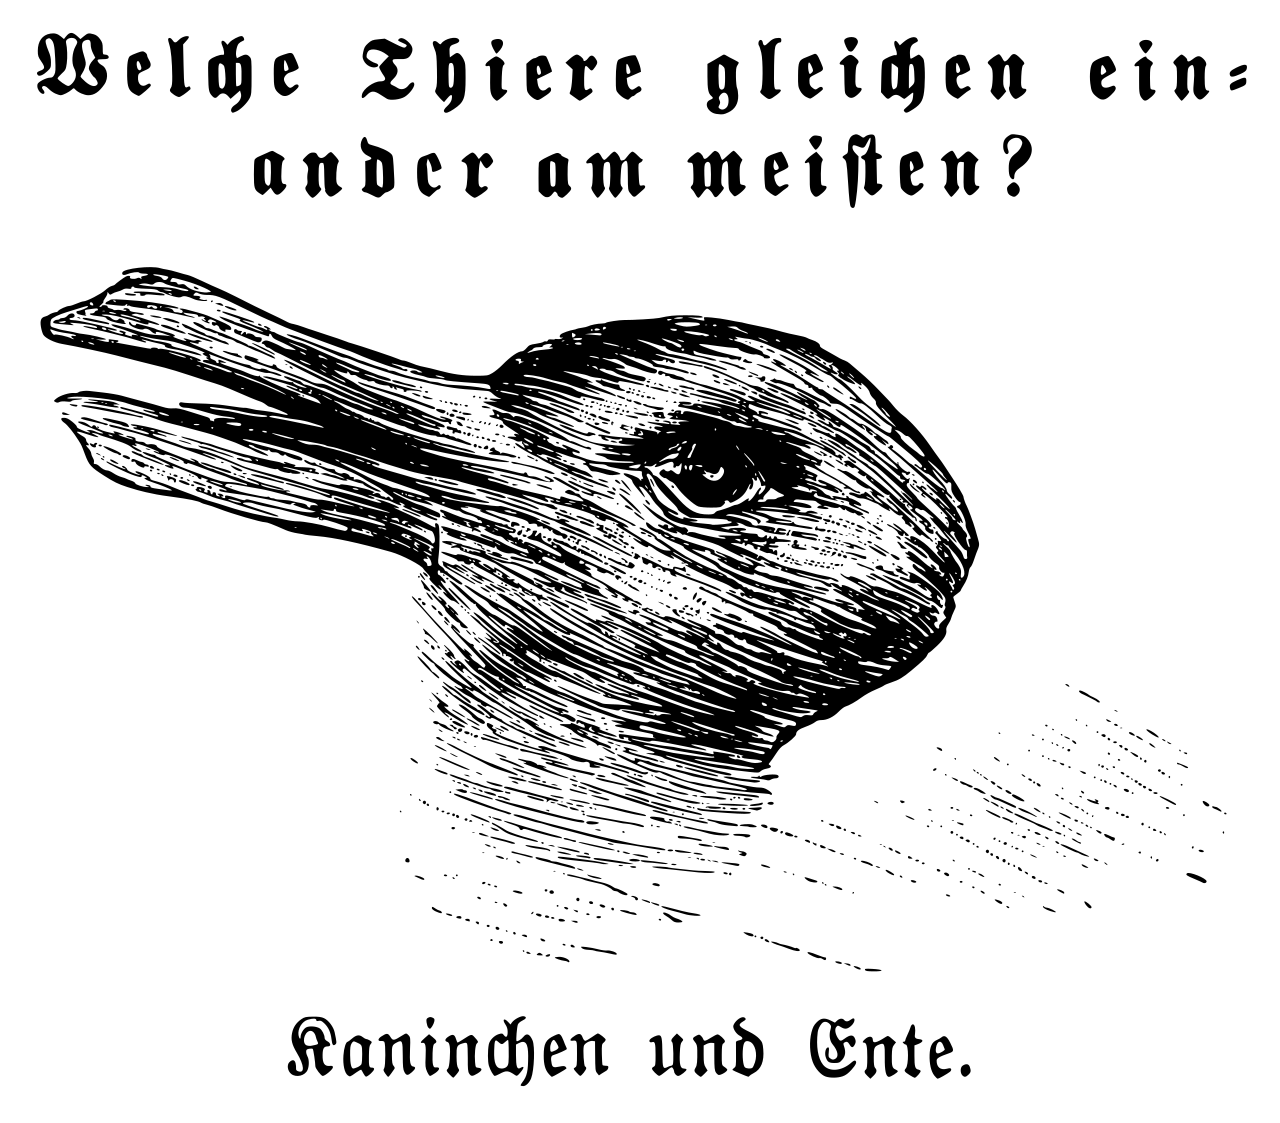
\includegraphics[width=0.5\textwidth]{images/rabbit_duck.png}
  \caption{"Kaninchen und Ente" (``Rabbit and Duck") from the 23 October 1892 issue of Fliegende Blätter}
  \label{fig: duck-rabbit}
\end{figure}
The concept was used by the Polish psychologist Joseph Jastrow, before the image was made famous by the Austrian philosopher Ludwig Wittgenstein. This image may seem like a digression in this discussion on learning without data collection, but it is not. Indeed, it illustrate that the focus of attention also has its limitations. In figure \ref{fig: duck-rabbit}, our attention is focused on the duck-rabbit's head, but we are not able to tell whether it represents a rabbit or a duck. In this case, some temporal context coupled with the notion of motion invariance from section \ref{sec: motion invariance} would be necessary to identify the animal. \\
This example shows that in some ambiguous, restricted (\eg if we only see the duck-rabbit's head) cases, the focus of attention is not sufficient to identify the object. As such, we can conclude that the focus of attention, although it may be necessary, is not sufficient for perfect recognition in all cases.

\section{Conclusion}
Let us leave the reader with a closing word after this discussion on ``Learning without data collection''. We saw that although the performances of deep learning are impressive, there is still a lot of room for improvement, especially when it comes to efficiency with respect to data quantities. As such, we came to state that deep learning is both better performing (in terms of accuracy) and worse performing (in terms of data efficiency) than humans. We saw two paths that can help us close the gap between deep learning's efficiency and the efficiency of Humans.
\paragraph{Motion invariance} Motion invariance is the property of objects to not change drastically as they go through time. Neither in shape, nor in other physical properties. This is a gift of nature that Humans are able to use to achieve better efficiency than deep learning algorithms. However, motion invariance is not sufficient for perfect recognition in all cases as we saw with the example of the jaguar which is identifiable only when it starts moving. We also saw the example of the frog which is not able to see what does not move. This example illustrates the fact that there has to be more than just motion invariance to achieve perfect recognition.
\paragraph{Focus of attention} The concept of focus of attention refers to the ability to selectively concentrate on specific aspects of the visual scene. We mentioned that some algorithms try to apply this concept to deep learning (namely Convolutional Neural Networks and Transformers). However, the amount of data needed for these networks to perform well proves that there is still a lot of room for efficiency improvements. We also saw that the focus of attention also has its limitations. In some ambiguous, restricted cases, such as the duck-rabbit's head, the focus of attention is not sufficient to identify the object. Thus we noted that the focus of attention may be necessary, but is not sufficient for perfect recognition in all cases.

Finally, we can only be sure of two things. First, deep learning has shown many impressive results, as well as great progress in the past decades. Second, there is still a lot of room for improvement in deep learning, especially in terms of efficiency. We know for sure that one achievable goal is to reach human-level efficiency. Most certainly, the next decades will be very interesting and show great improvements in terms of accuracy and efficiency of deep learning algorithms.



% \clearpage
% \printnoidxglossaries
\newpage
\begin{thebibliography}{99}
  \bibitem{gori2022} Betti, A., Gori, M. and Melacci, S., 2022. Deep Learning to See: Towards New Foundations of Computer Vision. arXiv preprint arXiv:2206.15351. 
  \bibitem{shen2019} Shen, L., Margolies, L.R., Rothstein, J.H., Fluder, E., McBride, R. and Sieh, W., 2019. Deep learning to improve breast cancer detection on screening mammography. Scientific reports, 9(1), p.12495. 
  \bibitem{lecun1995} LeCun, Y. and Bengio, Y., 1995. Convolutional networks for images, speech, and time series. The handbook of brain theory and neural networks, 3361(10), p.1995.
  \bibitem{vaswani2017} Vaswani, A., Shazeer, N., Parmar, N., Uszkoreit, J., Jones, L., Gomez, A.N., Kaiser, L. and Polosukhin, I., 2017. Attention is all you need. Advances in neural information processing systems, 30.
\end{thebibliography}
\end{document}

